\documentclass[a4paper]{article}
\usepackage[UTF8]{ctex}
\usepackage{geometry}
\usepackage{graphicx}
\usepackage{url}
\usepackage{multirow}
\usepackage{array}
\usepackage{booktabs}
\usepackage{url}
\usepackage{enumitem}
\usepackage{graphicx}
\usepackage{float}
\usepackage{amssymb}
\usepackage{amsmath}
\usepackage{subfig}
\usepackage{longtable}
\usepackage{pifont}
\usepackage{color} 

\allowdisplaybreaks

\geometry{a4paper, scale=0.78}

% \begin{figure}[H]
%     \centering
%     \includegraphics[width=.55\textwidth]{E.png}
%     \caption{矩阵与列向量的乘法}
%     \label{fig:my_label_1}
% \end{figure}

% \left\{
% \begin{array}{ll}
%       x+2x+z=2 & \\
%       3x+8y+z=12 & \\
%       4y+z=2
% \end{array}
% \right.

% \begin{enumerate}[itemindent = 1em, itemsep = 0.4pt, parsep=0.5pt, topsep = 0.5pt]

% \end{enumerate}

%\stackrel{a}{\longrightarrow}

%\underbrace{}_{} %下括号

%\tableofcontents %目录,并且目录页不记录页码
% \tableofcontents
% \newpage
% \setcounter{page}{1} %new page
% \clearpage

\title{Hidden Markov Model 05 Conclusion}
\author{Chen Gong}
\date{11 January 2020}

\begin{document}
\maketitle
Hidden Markov Model实际上是一个Dynamic Model。我们以Guassian Mixture Model (GMM)为例。对于一个观测状态,在隐变量状态给定的情况下,是符合一个Gaussian Distribution,也就是$D(O|i_1)\sim \mathcal{N}(\mu,\Sigma)$。如果,加入了time的因素就是Hidden Markov Model,而其中$\{ i_1,i_2,\cdots,i_T \}$是离散的就行,这些我们在第一章的背景部分有过讨论。而观测变量$o_1$是离散的还是连续的都不重要。

\section{Hidden Markov Model简述}
Hidden Markov Model,可以用一个模型,两个假设和是三个问题来描述。一个模型就是指$\lambda = (\pi, \mathcal{A}, \mathcal{B})$。其中,$\pi$:指的是初始概率分布;$\mathcal{A}$:指的是状态转移矩阵;$\mathcal{B}$:指的是发射矩阵,也就是在已知隐变量的情况下,得到观测变量的概率分布。

两个假设:1. 齐次马尔可夫模型,马尔科夫性质中非常重要的一条。2. 观测独立假设,也就是观测变量只和当前的隐变量状态有关。

三个问题:1. Evaluation:$P(O|\lambda)$,也就是在在已知模型的情况下,求观测变量出现的概率。2. Learning:$\hat{\lambda} = \arg\max_{\lambda}P(O|\lambda)$,在已知观测变量的情况下求解隐马尔可夫模型的参数。3. Decoding:$P(I|O) = P(i_1,\cdots,i_t|o_1,\cdots,o_t)$,用公式的语言描述就是$\hat{I} = \arg\max_I P(I,O|\lambda)$。

\section{Dynamic Model}
Dynamic Model实际上就是一个State Space Model,通常我们可以将Dynamic Model的问题分成两类。第一类为Learning问题,即为,参数$\lambda$是未知的,通过数据来知道参数是什么;第二类就是Inference问题,也就是在$\lambda$未知的情况下,推断后验概率。实际上,我们需要求的就是$P(Z|X)$,其中$X=\{ x_1,x_2,\cdots,x_N \}$而数据之间是非i.i.d的。

Inference问题大概可以被我们分成四类,Filtering Problem;Smoothing;Prediction Problem;Decoding。

\subsection{Learning}
Learing问题中$\lambda$是已知的,$\lambda_{MLE} = \arg\max_{\lambda}P(X|\lambda)$。我们采用的是Baum Welch Algorithm,算法思想上和EM算法类似,实际上也是Forward-Backward算法。

\subsection{Inference}
这一小节中,我们将分别来介绍Filtering;Smoothing;Prediction;Decoding,四个问题。

\subsubsection{Decoding}
这里前面已经做出过详细的描述了,这里就不再展开进行描述了,主要可以概括为:在已知观测数据序列的情况下,求得出现概率最大的隐变量序列,被我们描述为:$Z = \arg\max_z P(z_1,\cdots,z_t|x_1,\cdots,x_t)$。我们使用的一种动态规划的算法,被称为Viterbi Algorithm。

\subsection{Evaluation}
在还有大家应该见得比较多的Prob of Evidence问题,也就是:$P(X|\theta) = P(x_1,\cdots,x_t
\theta)$。我们通俗的称之为证据分布,实际上就是我们前面讲到的Evaluation方法。也就是在已知参数的情况下,求观测数据序列出现的概率,用公式描述即为:$P(X|\theta) = P(x_1,x_2,\cdots,x_t|\theta)$。

\subsubsection{Filtering}
实际上是一个Online-Learning的过程,也就是如果不停的往模型里面喂数据,我们可以得到概率分布为:$P(z_t|x_1,\cdots,x_t)$。所以Filtering非常的适合与on-line update。我们要求的这个就是隐变量的边缘后验分布。为什么叫滤波呢?这是由于我们求的后验是$P(z_t|x_1,\cdots,x_t)$,运用到了大量的历史信息,比$P(z_t|x_t)$的推断更加的精确,可以过滤掉更多的噪声,所以被我们称为“过滤”。求解过程如下所示:
\begin{equation}
    P(z_t|x_{1:t}) = \frac{P(z_t,x_1,\cdots,x_t)}{P(x_1,\cdots,x_t)} = \frac{P(z_t,x_1:x_t)}{\sum_{z_t} P(z_t,x_1:x_t)} \propto P(z_t,x_1:x_t)
\end{equation}

\subsubsection{Smoothing}
Smoothing问题和Filtering问题的性质非常的像,不同的是,Smoothing问题需要观测的是一个不变的完整序列。对于Smoothing问题的计算,前面的过程和Filtering一样,都是:
\begin{equation}
    P(z_t|x_{1:T}) = \frac{P(z_t,x_1,\cdots,x_T)}{P(x_1,\cdots,x_T)} = \frac{P(z_t,x_1:x_T)}{\sum_{z_t} P(z_t,x_1:x_T)} \propto P(z_t,x_1:x_T)
\end{equation}
同样因为$\sum_{z_t} P(z_t,x_1:x_T)$是一个归一化常数,我们这里不予考虑。下面的主要问题是关于$P(z_t,x_1:x_T)$如何计算,我们来进行推导:
\begin{equation}
    \begin{split}
        P(x_{1:T},z_t) = & P(x_{1:t},x_{t+1:T},z_t) \\
        = & P(x_{t+1:T}|x_{1:t},z_t) \cdot \underbrace{P(x_{1:t},z_t)}_{\alpha_t}
    \end{split}
\end{equation}

推导到了这里就是要对$P(\underbrace{x_{t+1:T}}_{C}|\underbrace{x_{1:t}}_{A},\underbrace{z_t}_{B})$进行分析,在这个概率图模型中,符合如下结构:
\begin{figure}[H]
    \centering
    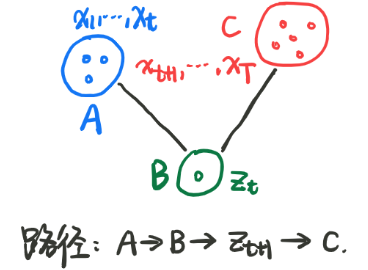
\includegraphics[width=.45\textwidth]{微信图片_20200110123017.png}
    \caption{A,B,$z_{t+1}$,C,概率图结构图}
    \label{fig:my_label_1}
\end{figure}

根据概率图模型中提到D-Separation中,我们可以很简单的得出,$A\perp C|B$。所以,$P(x_{t+1:T}|x_{1:t},z_t) = P(x_{t+1:T}|x_{1:t},z_t = \beta_t)$。所以,我们可以得到:
\begin{equation}
    P(x_{1:T},z_t) = \alpha_t \cdot \beta_t
\end{equation}

那么,最终得到的就是:
{\color{red}
\begin{equation}
    P(z_t|x_{1:T}) \propto P(x_{1:T},z_t) = \alpha_t\beta_t
\end{equation}
}

所以,我们需要同时用到Forward Algorithm和Backward Algorithm,所以,被我们称为Forward-Backward Algorithm。

\subsubsection{Prediction}
预测问题,大体上被我们分成两个方面:
\begin{equation}
    \begin{split}
        P(z_{t+1}|x_1,\cdots,x_t) = & \sum_{z_t} P(z_{t+1},z_t|x_1,\cdots,x_t) \\ 
        = & \sum_{z_t} \underbrace{P(z_{t+1}|z_t, x_1,\cdots,x_t)}_{P(z_{t+1}|z_t)} \underbrace{P(z_t|z_t, x_1,\cdots,x_t)}_{Filtering} \\
    \end{split}
\end{equation}
\begin{equation}
    \begin{split}
        P(x_{t+1}|x_1,\cdots,x_t) 
        = & \sum_{z_{t+1}} P(x_{t+1},z_{t+1}|x_1,\cdots,x_t) \\ 
        = & \underbrace{P(x_{t+1}|z_{t+1},x_1,\cdots,x_t)}_{P(x_{t+1}|z_{t+1})} \cdot \underbrace{P(z_{t+1}|x_1,\cdots,x_t)}_{Formula (6)}
    \end{split}
\end{equation}

公式(7)选择从$z_{t+1}$进行积分的原因是因为想利用齐次马尔科夫性质。实际上求解的过程大同小异都是缺什么就补什么。

其实,我们已经大致的介绍了Dynamic Model的几种主要模型,后面我们会详细的来解释线性动态系统。






\end{document}